\chapter{Standard Construction and Destruction Algorithms \Author{\chapternewline J.~Singer \andAuthor F.~Rastello}}
\label{chapter:classical_construction_algorithm}
\inputpath{part1}{classical_construction_algorithm}
\inputprogress


{ 
%% jsinger - simple introductory paragraphs

This chapter \index{SSA!construction}\index{SSA!destruction}%
describes the standard algorithms for construction and
destruction of SSA form.
%
SSA \emph{construction} refers to the process of translating a non-SSA program into
one that satisfies the SSA constraints. In general, this transformation
occurs as one of the
earliest phases in the middle-end of an optimizing compiler, when the program
has been converted to three-address intermediate code.
SSA \emph{destruction} is sometimes called out-of-SSA translation. This step
generally
takes place in an optimizing compiler after all SSA optimizations have
been performed, and prior to code generation. Note however that there are
specialized code generation techniques that can work directly on SSA-based
intermediate representations such as instruction selection (see
Chapter~\ref{chapter:code_selection}), if-conversion (see
Chapter~\ref{chapter:if_conversion}),
and register allocation (see Chapter~\ref{chapter:register_allocation}).

The algorithms presented in this chapter are
based on material from the seminal research papers on SSA.
These original algorithms are 
straightforward to implement and have acceptable efficiency.
Therefore such algorithms
are widely implemented in current compilers.
Note that more
efficient, albeit more complex, alternative algorithms have been devised.
These are described further in Chapters 
\ref{chapter:alternative_ssa_construction_algorithms}
and
\ref{chapter:alternative_ssa_destruction_algorithm}.

% To be put in vanilla if necessary
%% Throughout this chapter,
%% we assume that a `program' is represented as an
%% intra-procedural control-flow graph (CFG)
%% with a single entry node $r$, from which every other
%% node is reachable.
%% Each node is a basic block, containing a straightline
%% sequence of program statements.
%% Data flow occurs through definitions and uses of 
%% variables, with no pointer indirection.
%% %% FIXME - forward reference to Part II ...
%% (Part II of this textbook contains chapters dealing with
%% SSA extensions for high-level features like
%% pointer-based aliasing, arrays, compound data structures, concurrency, etc.)

Figure~\ref{fig:classical_construction_algorithm:examplecfg}
shows the control-flow graph (CFG) of an example
program. The set of nodes is $\{ r, A, B, C, D, E\}$, and
the variables used are $\{ x, y, \textit{tmp} \}$.
Note that the program shows the complete control-flow structure,
denoted by directed edges between the nodes.
However, the program only shows 
statements that define relevant variables, together with the
unique \texttt{return} statement at the exit point of the CFG.
All of the program variables are undefined on entry. On certain
control-flow paths, some variables may be used without being defined, 
e.g.\ $x$ on the path $r \rightarrow A \rightarrow C$. 
We discuss this issue later in the chapter.
We intend to use this program as a running example
throughout the chapter,
to demonstrate various aspects of SSA construction.


\begin{figure}
  \begin{center}
    \tikzsubfigure[1]{initial}
  \end{center}
\caption{\label{fig:classical_construction_algorithm:examplecfg}Example control-flow graph, before
  SSA construction occurs.}
\end{figure}

\section{Construction}
\label{sec:classical_construction}

The original construction algorithm for SSA form 
consists of two distinct phases.
\begin{enumerate}
\item \textbf{\phifun\ insertion}\index{insertion, of \phifun} performs \textit{live-range splitting}\index{live-range splitting} to ensures that any use of a given variable $v$ is reached\footnote{A program point $p$ is said to be \emph{reachable} by a definition of $v$ if there exists a path in the CFG from that definition to $p$ that does not contain any other definition of $v$.}\index{reachable, by a definition}  by exactly one definition of $v$. 
The resulting live-ranges exhibit the property of having a single definition, which occurs at the beginning of each live-range.\index{live-range}\index{single definition property}
\item \textbf{Variable renaming}\index{renaming, of variables} assigns a unique variable name\index{variable name} to each live-range. This second phase rewrites variable names in program statements such that the program text contains only one definition of each variable, and every use refers to its corresponding unique reaching definition.
\end{enumerate}

As already outlined in Chapter~\ref{chapter:properties_and_flavours},
there are different flavors of SSA with distinct properties.
In this chapter, we focus on the \textit{minimal} SSA form\index{minimal SSA form}.

\subsection{Join Sets and Dominance Frontiers}

In order to explain how \phifun\ insertions occur,
it will be helpful 
to review the related concepts of \textit{join sets} and
\textit{dominance frontiers}.

For a given set of nodes $S$ in a CFG, the join set $\join(S)$\index{join set}
is the set of \textit{join nodes} of $S$,
i.e., nodes in the CFG that can be reached by
two (or more) distinct elements of $S$ using disjoint paths.
Join sets were introduced in Chapter~\ref{chapter:properties_and_flavours}, 
Section~\ref{sec:properties_and_flavors:minimality}.

Let us consider some join set examples from the
program in Figure~\ref{fig:classical_construction_algorithm:examplecfg}.
\begin{enumerate}
\item $\join(\{B,C\}) = \{D\}$, since it is possible to get from $B$ to $D$
and from $C$ to $D$ along different, non-overlapping, paths.
\item Again, $\join(\{r, A, B, C, D, E \}) = \{A,D,E\}$, since the nodes
$A$, $D$, and $E$ are the only nodes with multiple predecessors in
the program.
\end{enumerate}


% Chapter 2 defers definition of dominance frontiers
% until here, and gives an explicit forward reference
% Recall the definition of dominance frontiers from Section~\ref{sec:properties_and_flavors:minimalSSA}.
The \textit{dominance frontier}\index{dominance frontier, DF} of a node $n$,
$\DF(n)$, is the border of the CFG region that is dominated by $n$.
More formally,
\begin{itemize}
\item node $x$ \textit{strictly dominates}\index{dominates, strictly} node $y$ if $x$ dominates
  $y$ and $x \neq y$;
\item the set of nodes $\DF(n)$ contains all nodes $x$ such that $n$
  dominates a predecessor of $x$ but $n$ does not strictly dominate $x$.
\end{itemize}

For instance, in our 
Figure~\ref{fig:classical_construction_algorithm:examplecfg}, the dominance 
frontier of the $y$ defined in block B is the first operation of D, while the 
$\DF$ of the $y$ defined in block C would be the first operations 
of D and E.


Note that $\DF$ is defined over individual nodes, 
but for simplicity of presentation, we overload it to 
operate over sets of nodes too, i.e., 
$\DF(S) = \bigcup_{s\in S} \DF(s)$.
The \textit{iterated dominance frontier} $\iDF(S)$\index{iterated dominance 
frontier, \iDF} is obtained by iterating the computation of $\DF$ until 
reaching a fixed point, i.e., it is the limit 
$DF_{i\rightarrow\infty}(S)$
of the sequence:
$$\begin{array}{lll}
\DF_1(S) & = & \DF(S)\\
\DF_{i+1}(S) & = & \DF\left(S\cup \DF_i(S)\right)
\end{array}$$


Construction of minimal SSA 
requires for each variable $v$ the insertion of \phifuns\ at $\join(\defsv)$,
where $\defsv$ is the set of nodes that contain definitions of $v$.
The original construction algorithm
for SSA form uses the iterated dominance frontier $\iDF(\defsv)$.
This is an over-approximation of join set, since
$\iDF(S)=\join(S\cup \{r\})$,
i.e., the original algorithm assumes an \emph{implicit} definition of every
variable at the entry node $r$.


\subsection{\phifun\ Insertion}

This concept of dominance frontiers 
naturally leads to a
straightforward approach that places \phifuns\
on a per-variable basis.
For a given variable $v$, we place \phifuns\ at the
iterated dominance frontier $\iDF(\defsv)$ where
$\defsv$ is the set of nodes containing definitions of $v$.
This leads to the construction of SSA form that has 
the dominance property\index{dominance property}, i.e., where each the 
definition of each renamed variable dominates its entire live-range.

Consider again our running example from Figure~\ref{fig:classical_construction_algorithm:examplecfg}. The set of nodes containing definitions
of variable
$x$ is $\{ B,C,D \}$. The iterated dominance frontier of this set 
is $\{ A, D, E \}$ (it is also the $\DF$, no iteration needed here). Hence we need to insert 
\phifuns\ for $x$ at the beginning of nodes $A$, $D$, and $E$.
Figure~\ref{fig:classical_construction_algorithm:examplecfg_varx} shows the example CFG program
with \phifuns\ for $x$ inserted.

\begin{figure}
  \tikzsubfigure[2]{initial}
\caption{\label{fig:classical_construction_algorithm:examplecfg_varx}Example control-flow graph, including
inserted \phifuns\ for variable $x$.
}
\end{figure}



As far as the actual algorithm for \phifuns\ insertion
is concerned, we will assume that the dominance
frontier of each CFG node is pre-computed and that the iterated dominance 
frontier is computed on the fly, as the algorithm proceeds.
The algorithm works by inserting \phifuns\ iteratively
using a worklist of definition points, and flags (to avoid multiple
insertions). The corresponding pseudo-code for
\phifun\ insertion is given in
Algorithm~\ref{alg:classical_construction:phi_insertion}.
%
The worklist of nodes $W$ is used to record definition points that the
algorithm
has not yet processed, i.e., it has not yet inserted \phifuns\ at their dominance
frontiers.
Because a \phifun\ is itself a 
definition, it may require further \phifuns\ to be inserted.
This is the cause of node insertions into the worklist $W$ during
iterations of the inner loop in Algorithm 
\ref{alg:classical_construction:phi_insertion}.
Effectively, we compute the iterated dominance frontier on the fly.
%
The set $F$ is used to avoid repeated insertion of \phifuns\
on a single block. Dominance
frontiers
of distinct nodes may intersect, e.g., in the example CFG in Figure
\ref{fig:classical_construction_algorithm:examplecfg},
$\DF(B)$ and $\DF(C)$ both contain $D$, but
once a \phifun\ for a particular variable has been
inserted at a node,
there is no need to insert another, since a single \phifun\ per
variable handles all incoming definitions of that variable to that node.


%%%
%  Seems there is a problem, F should be emptied for a new v
%%%
\begin{algorithm}[h]
  $F \leftarrow \{ \}$\tcc*[r]{set of basic blocks where $\phi$ is added}
  \For{$v$: variable names in original program}{
     $W \leftarrow \{ \}$\tcc*[r]{set of basic blocks}
     \For{$d \in \defsv$ }{
       \textbf{let} $B$ be the basic block containing $d$\;
       $W \leftarrow W \cup \{ B \}$\;
   }
   \While{$W \neq \{\}$}{
     remove a basic block $X$ from $W$\;
     \For{$Y$: $\mbox{basic block} \in \mathrm{DF}(X)$}{
       \If{$Y \not\in F$}{
         add $v \leftarrow \phi(...)$ at entry of $Y$\;
         $F \leftarrow F \cup \{ Y \}$\;
         \If{$Y \notin \defsv$}{
           $W \leftarrow W \cup \{ Y \}$\;
         }
       }
    }
  }
}
\caption{\label{alg:classical_construction:phi_insertion}Standard algorithm for 
inserting $\phi$-functions for  a variable $v$.}
\end{algorithm}

We give gives a walkthrough example of 
Algorithm~\ref{alg:classical_construction:phi_insertion} in
Table~\ref{table:classical_construction:walkthru}. 
It shows the stages of execution for a single iteration of
the outermost for loop, inserting \phifuns\
for variable $x$.
Each row represents a single iteration of the while loop
that iterates over the worklist $W$. The table shows the values
of $X$, $F$ and $W$ at the start of each while loop iteration.
At the beginning, the CFG looks like Figure~\ref{fig:classical_construction_algorithm:examplecfg}.
At the end, when all the \phifuns\ for $x$ have
been placed, then the CFG looks like Figure~\ref{fig:classical_construction_algorithm:examplecfg_varx}.



\begin{table}
  {\def\sp{@{\kern1.5em}}
\begin{center}
  \begin{tabular}{c\sp c\sp c\sp c\sp c}
\textbf{while loop \#} & $X$ & $\DF(X)$ & $F$         & $W$\\ \hline
-                      & -   & -                & $\{\}$      & $\{B,C,D\}$ \\
1                      & $B$ & $\{D\}$          & $\{D\}$     & $\{C,D\}$ \\
2                      & $C$ & $\{D,E\}$        & $\{D,E\}$   & $\{D,E\}$ \\
3                      & $D$ & $\{E,A\}$        & $\{D,E,A\}$ & $\{E,A\}$\\
4                      & $E$ & $\{\}$           & $\{D,E,A\}$ & $\{A\}$\\
5                      & $A$ & $\{A\}$          & $\{D,E,A\}$ & $\{\}$\\ 
\end{tabular}
\end{center}
}
\caption{\label{table:classical_construction:walkthru} Walkthrough of
  placement of \phifuns\ for variable $x$ in example CFG.}
\end{table}


Providing the dominator tree is given, the computation of the dominance frontier is quite straightforward. As illustrated by Figure~\ref{fig:classical_construction_algorithm:iDF}, this can be understood using the DJ-graph notation. The skeleton of the \DJ-graph\index{DJ-graph@\DJ-graph} is the dominator tree of the CFG that makes the D-edges\index{dominance edge, D-edge} (dominance edges). This is augmented with J-edges (join edges)\index{join edge, J-edge} that correspond to all edges of the CFG whose source does not strictly dominate its destination. A \DF-edge (dominance frontier edge)\index{dominance frontier edge, DF-edge} is an edge whose destination is in the dominance frontier of its source. By definition, there is a \DF-edge $(a,b)$ between every CFG nodes $a$, $b$ such that $a$ dominates a predecessor of $b$, but does not strictly dominate $b$. 
In other-words, for each  $J$-edge $(a,b)$, all ancestors of $a$ (including
$a$) that do not strictly dominate $b$ have $b$ in their dominance
frontier. For example, in Figure~\ref{fig:classical_construction_algorithm:iDF}, $(F,G)$ is a J-edge, so $\{(F,G),\ (E,G),\ (B,G)\}$ are \DF-edges. This leads to the pseudo-code given in
Algorithm~\ref{alg:classical_construction:df}, where for every edge $(a,b)$ we visit all ancestors of 
$a$ to add $b$ to their dominance frontier.
 
Since the iterated dominance frontier is simply the transitive closure
of the dominance frontier, we can define the \iDF-graph as the transitive closure of the \DF-graph. In our example, as $\{(C,E),\ (E,G)\}$ are \DF-edges, $(C,G)$ is a \iDF-edge. Hence, a definition of $x$ in $C$ will lead to inserting \phifuns in $E$ and $G$.
We can compute the iterated dominance frontier for each variable independently, as outlined in this chapter, or ``cache'' it to avoid repeated computation of the iterated dominance frontier of the same node. This leads to more sophisticated algorithms detailed in Chapter~\ref{chapter:alternative_ssa_construction_algorithms}.

\begin{figure}
  \subfloat[CFG]{
    \tikzfigure{iDF-CFG}
  }
  \subfloat[\DJ-graph]{\label{fig:classical_construction_algorithm:iDF-J}
    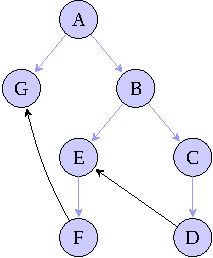
\includegraphics[scale=0.7]{tikz/iDF-J.pdf}
  }
  \subfloat[\DF-graph]{
    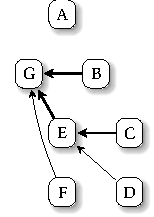
\includegraphics[scale=0.7]{tikz/iDF-DF.pdf}
  }
  \subfloat[\iDF-graph]{
    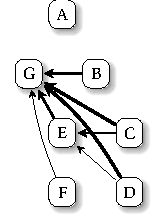
\includegraphics[scale=0.7]{tikz/iDF-iDF.pdf}
  }
\caption{\label{fig:classical_construction_algorithm:iDF}An example CFG and its 
corresponding DJ-graph ($D$-edges are top-down), \DF-graph and \iDF-graph.}
\end{figure}

\begin{algorithm}
 \For{$(a,b) \in \mathrm{CFG\ edges}$}{
  $x \leftarrow a$\;
  \While{x does not strictly dominate b}{
     $\DF(x) \leftarrow \DF(x) \cup b$\;
     $x \leftarrow \mathrm{immediate\ dominator}(x)$\;
  }
 }
\caption{\label{alg:classical_construction:df}Algorithm for computing the 
dominance frontier of each CFG node.}\index{dominance frontier, construction}
\end{algorithm}



Once \phifuns\ have been inserted using this algorithm, the program usually
still contains several definitions per variable, however, now there is a
single definition statement in the CFG that reaches each use.  
For each variable use in a \phifun, it is conventional to treat them as if the 
use actually occurs on the corresponding incoming edge or at the end of the
corresponding predecessor node.
If we follow this convention,  
% Moreover, with the following semantics for \phifuns\ where its
% variable uses are considered to be on the corresponding predecessor
% basic blocks,
then def-use chains\index{def-use chains} are aligned with the CFG dominator tree.
In other words,
\emph{the single definition that reaches each use dominates that use}.

\subsection{Variable Renaming}
\index{renaming, of variables}
\newcommand\reachingDef[1]{#1.\mathrm{reachingDef}}
To obtain the desired property of a static single assignment per variable,
it is necessary to perform variable renaming, which
is the second phase in the SSA construction process.
\phifun\ insertions have the effect of splitting the live-range(s)\index{live-range splitting} of
each original variable into pieces. The variable renaming phase
associates to each individual live-range a new variable name, also
called a \emph{version}.\index{variable!version}\index{variable!name}
The pseudo-code for this process is presented in 
Algorithm~\ref{alg:classical:renaming}.
Because of the dominance property outlined above,
it is straightforward to rename variables
using a depth-first traversal of the dominator tree.
During the traversal, for each variable $v$, it is necessary to
remember the version of its unique reaching definition at some point $p$ in
the graph. This corresponds to the closest definition that dominates $p$.
In Algorithm~\ref{alg:classical:renaming}, we compute and cache the 
reaching definition for $v$ in the per-variable slot ``$\reachingDef{v}$''
that is updated as the algorithm traverses the dominator tree of the
SSA graph.
This per-variable slot 
% This renaming algorithm uses a single $\mathrm{reachingDef}$ slot 
stores the in-scope, ``new'' variable name (version) for the equivalent
variable at the same point in the un-renamed program.

\begin{algorithm}
%proc renaming:
\tcc{rename variable definitions and uses to have one definition per
  variable name}
\ForEach{v : Variable}{
    $\reachingDef{v} \leftarrow \bot$\;
}
\ForEach{ \textit{BB} : basic Block in depth-first search preorder traversal of the dominance tree}{
  \ForEach{ i : instruction in linear code sequence of \textit{BB}}{
      \ForEach{v : variable used by non-\phifun\ i}{
        $\mathrm{updateReachingDef}(v,i)$\;
        replace this use of $v$ by $\reachingDef{v}$ in $i$\;
      }
      \ForEach{ v : variable defined by i (may be a \phifun)}{
        $\mathrm{updateReachingDef}(v,i)$\;
        create fresh variable $v'$\;
        replace this definition of $v$ by $v'$ in $i$\;
        $\reachingDef{v'} \leftarrow \reachingDef{v}$ \;
        $\reachingDef{v} \leftarrow v'$\;
      }
  }
  \ForEach{$\phi$: \phifun\ in a successor of \textit{BB}}{
      \ForEach{ v : variable used by $\phi$}{
        $\mathrm{updateReachingDef}(v,\phi)$\;
        replace this use of $v$ by $\reachingDef{v}$ in $\phi$\;
      }
 }
}
\caption{\label{alg:classical:renaming}Renaming algorithm for second
  phase of SSA construction}\index{renaming, of variable.}
\end{algorithm}

The variable renaming algorithm translates our running example 
from Figure~\ref{fig:classical_construction_algorithm:examplecfg}
into the SSA form of Figure~\ref{fig:classical_construction_algorithm:renaming}. 
The table in Figure~\ref{table:classical_construction_algorithm:renaming} 
gives a walkthrough example of Algorithm~\ref{alg:classical:renaming},
only considering variable $x$. The labels $l_i$ mark
instructions in the program that mention $x$, shown in 
Figure~\ref{fig:classical_construction_algorithm:renaming}.
The table records (1) when $\reachingDef{x}$ is updated
from $x_\mathrm{old}$ into
$x_\mathrm{new}$ due to a call of updateReachingDef,
and (2) when $\reachingDef{x}$ is $x_\mathrm{old}$ before
a definition statement, then $x_\mathrm{new}$ afterwards.

\begin{figure}
\subfloat[CFG]{
  \tikzsubfigure[3]{initial}
\label{fig:classical_construction_algorithm:renaming}
}\hfill
\subfloat[Walk-trough of renaming for variable $x$]
{
\def\u#1{\hphantom{def} $l_#1$ use}
\def\d#1{def $l_#1$ \hphantom{use}}
\def\k{@{\kern4pt}}
\begin{tabular}[b]{c\k|\k c\k |\k l}
\textit{BB} & $x$ mention &  $\reachingDef{x}$ \\ \hline
$r$ & \u{1} & $\bot$\\
$A$ & \d{1} &  $\bot$ then $x_1$\\
$B$ & \d{2} &  $x_1$ then $x_2$\\
$B$ & \u{5} & $x_2$\\
$C$ & \u{3} & $x_2$ updated into $x_1$\\
$C$ & \d{4} &  $x_1$ then $x_3$\\
$C$ & \u{5} & $x_3$\\
$C$ & \u{7} & $x_3$\\
$D$ & \d{5} & $x_3$ updated into $x_1$ then $x_4$\\
$D$ & \u{6} & $x_4$\\
$D$ & \d{6} & $x_4$ then $x_5$\\
$D$ & \u{1} & $x_5$\\
$D$ & \u{7} & $x_5$\\
$E$ & \d{7} & $x_5$ then $x_6$\\
$E$ & \u{8} & $x_6$\\
\end{tabular}\label{table:classical_construction_algorithm:renaming}
}
\caption{SSA form of the example of 
Figure~\ref{fig:classical_construction_algorithm:examplecfg}.}
\end{figure}


\begin{procedure}
\KwData{$v$ : variable from program}
\KwData{$i$ : instruction from program}
  \tcc{search through chain of definitions for v until we find the
    closest definition that dominates i, then update $\reachingDef{v}$
    in-place with this definition}
  $r \leftarrow \reachingDef{v}$\;
  \While{ not ($r==\bot$ or definition($r$) dominates $i$)}{
    $r \leftarrow \reachingDef{r}$\;
  }
  $\reachingDef{v} \leftarrow r$\;
\caption{updateReachingDef(v,i) Utility
  function for SSA renaming\label{alg:classical:updateRD}}\index{reaching 
  definition.}
\end{procedure}

% Some paragraphs summarizing similarities / diffs between this
% algorithm and standard stack-based renaming algorithm.
The original presentation of the renaming algorithm uses
a per-variable stack that stores
all variable versions that dominate the current program
point, rather than the slot-based approach outlined above.
%
In the stack-based algorithm, 
a stack value is pushed when a variable definition is
processed (while we explicitly update the reachingDef field at this point).
The top stack value is peeked when a variable use is encountered
(we read from the reachingDef field at this point).
Multiple stack values may be popped when moving to a different node
in the dominator tree 
(we always check whether we need to update the reachingDef field
before we read from it).
%
While the slot-based algorithm requires more memory, it can take advantage of 
an existing working field for a variable, and be more efficient in practice. 

\subsection{Summary}

Now let us review the flavour of SSA form that this simple
construction algorithm produces. We refer back to several
SSA properties that were introduced in
Chapter~\ref{chapter:properties_and_flavours}.

\begin{itemize}
\item It is \textit{minimal} (see~Section~\ref{sec:properties_and_flavors:minimality}).\index{minimal SSA form}
After the \phifun\ insertion phase,
but before variable renaming, the CFG contains the minimal 
number of inserted \phifuns\ to achieve the property that exactly
one definition of each variable $v$ reaches every point in the graph.
\item It is \textit{not pruned} (see Section~\ref{sec-prop-pruned}).\index{pruned SSA form}
Some of the inserted \phifuns\
may be dead, i.e., there is not always an explicit use of the variable subsequent
to the \phifun (e.g., $y_5$ in Figure~\ref{fig:classical_construction_algorithm:renaming}).
\item It is \textit{conventional} (see Section~\ref{sec-prop-conventional}).\index{conventional SSA form, CSSA}
The transformation that renames all $\phi$-related variables into a
unique representative name and then removes all \phifuns\ is a correct SSA-destruction algorithm.
\item Finally, it has the \textit{dominance} property (see Section
\ref{sec:properties_and_flavours:domprop}).\index{strict SSA form}\index{dominance property, SSA form with}
Each variable use is dominated by its unique definition. 
This is due to the use of iterated dominance frontiers
during the $\phi$-placement phase,
rather than join sets. Whenever the iterated dominance frontier
of the set of definition points of a variable differs from its join
set, then at least one program point can be reached both by $r$ (the
entry of the CFG) and one of the definition points. In other words, as
in Figure~\ref{fig:classical_construction_algorithm:examplecfg}, one
of the uses of the \phifun\ inserted in block $A$ for $x$ does not have
any actual reaching definition that dominates it. This corresponds to
the $\valundef$ value used to initialize each reachingDef slot in Algorithm\index{undefined variable}
\ref{alg:classical:renaming}.
Actual implementation code can use a \texttt{NULL} value, create a
fake undefined variable at the entry of the CFG, or create
undefined pseudo-operations on-the-fly just before the particular use.
% We choose to use in this book the undef value, represented with the $\undef$ sign.
\end{itemize}


\section{Destruction}
\label{sec:classical_construction_algorithm:destruction}
\index{SSA destruction}
SSA form is a sparse representation of program information,
which enables simple, efficient code analysis and optimization.
Once we have completed SSA based optimization passes,
and certainly before code generation,
it is necessary to eliminate \phifuns\ since these
are not executable machine instructions.
This elimination phase is known as \textit{SSA destruction}. 

When freshly constructed, an untransformed SSA code is conventional and its destruction is straightforward:\index{conventional SSA form}
One simply has to rename all 
$\phi$-related variables (source and destination operands of
the same \phifun)
into a unique representative variable.
Then, each \phifun\ should have syntactically identical
names for all its operands,
and thus can be removed to coalesce the related live-ranges.\index{coalescing, of variables}

We refer to a set of $\phi$-related variables as
a \phiweb.\index{\phiweb} We recall from
Chapter~\ref{chapter:properties_and_flavours}
that conventional SSA is defined as a flavor under which each
\phiweb is free from interferences.
Hence, if all variables of a \phiweb\index{conventional SSA}
have non-overlapping live-ranges then the SSA form is conventional.
The discovery of \phiwebs can be performed efficiently 
using the classical \textit{union-find} algorithm 
with a disjoint-set data structure,
which keeps track of a set of elements
partitioned into a number of disjoint (non-overlapping) subsets.
The \phiwebs discovery algorithm is presented in 
Algorithm~\ref{alg:ssadestruction:find-webs}.

\begin{algorithm}
%% proc find_webs
%% // find the ssa web of each variable
\Begin{
\For{each variable $v$}{
  $\mathrm{phiweb}(v) \leftarrow \{v\}$;
}
\For{each instruction of the form $a_{\mathrm{dest}} = \phi(a_1,\ldots,a_n)$}{
  \For{each source operand $a_i$ in instruction}{
     union$(\mathrm{phiweb}(a_{\mathrm{dest}}),\mathrm{phiweb}(a_i))$
  }
}
}
\caption{\label{alg:ssadestruction:find-webs}The \phiwebs discovery algorithm, 
based on the union-find pattern}\index{\phiweb, discovery.}
\end{algorithm}


While freshly constructed SSA code is conventional, 
this may not be the case after performing some optimizations 
such as copy propagation.
Going back to conventional SSA form requires the insertion of copies.
%
The simplest (although not the most efficient) way to destroy non-conventional SSA form is to split all \textit{critical edges}, and then replace \phifuns\ by copies\index{parallel copy} at the end of predecessor basic blocks. 
A critical edge is an edge from a node with several successors to a node with several predecessors.\index{critical edge}
The process of splitting an edge\index{edge splitting}, say $(b_1,b_2)$,
involves replacing edge $(b_1, b_2)$ by (i) an
edge from $b_1$ to a freshly created basic block 
and by (ii) another edge from this fresh basic block to $b_2$. 
As \phifuns have a parallel semantic, i.e., have to be executed simultaneously not sequentially, the same holds for the corresponding copies inserted at the end of predecessor basic blocks. To this end, a pseudo instruction called a \emph{parallel copy}\index{parallel copy} is created to represent a set of copies that have to be executed in parallel.
The replacement of parallel copies by sequences of simple copies is handled later on.
Algorithm~\ref{alg:ssadestruction:splitting} presents
the corresponding pseudo-code that makes non-conventional SSA conventional. \index{transformed SSA, T-SSA}\index{conventional SSA, C-SSA}
As already mentioned, SSA destruction of such form is straightforward. However, 
Algorithm~\ref{alg:ssadestruction:splitting} can be slightly modified to 
directly destruct SSA by deleting line~\ref{line:api}, replacing $a'_i$ by $a_0$ in the 
following lines, and adding ``remove the \phifun'' after them.

%  \LinesNotNumbered
\begin{algorithm}
\LinesNumbered
\Begin{
 \ForEach{$B$: basic block of the CFG}{
   \Let{$(E_1,\ldots,E_n)$ be the list of incoming edges of $B$}\;
   \ForEach{$E_i=(B_i,B)$}{
     \Let{$\mathrm{PC}_i$ be an empty parallel copy instruction}\;
     \If{$B_i$ has several outgoing edges}{
       create fresh empty basic block $B'_i$\;
       replace edge $E_i$ by edges $B_i \rightarrow B'_i$ and $B'_i \rightarrow B$\;
       insert $PC_i$ in $B'_i$\;
     }
    \Else{
       append $PC_i$ at the end of $B_i$\;
     }
   }
   \ForEach{\phifun\ at the entry of $B$ of the form $a_0=\phi(B_1:a_1,\ldots,B_n:a_n)$}{
     \ForEach{$a_i$ (argument of the \phifun\ corresponding to $B_i$)}{
%       \nl\Let{$a'_i$ be a freshly created variable}\label{line:api} \; %/!\ Label does not work so wrote in hard in the text
       \Let{$a'_i$ be a freshly created variable}\nllabel{line:api} \; %/!\ Label does not work so wrote in hard in the text
       add copy $a'_i \leftarrow a_i$ to $\mathrm{PC}_i$\;
       replace $a_i$ by $a'_i$ in the \phifun\;
     }
%     \nl\BlankLine\label{line:removephi} %/!\ same
     \BlankLine\nllabel{line:removephi} %/!\ same
  }
}
}
\caption{\label{alg:ssadestruction:splitting}Critical Edge Splitting Algorithm for making non-conventional SSA form conventional.}
\end{algorithm}



We stress that the above destruction technique has several drawbacks: first because of specific architectural constraints, region boundaries, or exception handling code, the compiler might not permit the splitting of a given edge\index{edge splitting}; second, the resulting code contains many temporary-to-temporary copy operations. In theory, reducing the frequency of these copies is the role of the coalescing during the register allocation phase. A few memory- and time-consuming coalescing heuristics mentioned in Chapter~\ref{chapter:register_allocation} can handle the removal of these copies effectively. Coalescing can also, with less effort, be performed prior to the register allocation phase. As opposed to a (so-called conservative) coalescing\index{conservative coalescing} during register allocation\index{register allocation}, this \emph{aggressive} coalescing\index{aggressive coalescing} would not cope with the interference graph colorability. Further, the process of copy insertion itself might take a substantial amount of time and might not be suitable for dynamic compilation. The goal of Chapter~\ref{chapter:alternative_ssa_destruction_algorithm} is to cope both with non-splittable edges and difficulties related to SSA destruction at machine code level, but also aggressive coalescing in the context of resource constrained compilation.

Once \phifuns\ have been replaced by parallel copies, we need to sequentialize the parallel copies, i.e., replace them by a sequence of simple copies. This phase can be performed immediately after SSA destruction or later on, perhaps even after register allocation (see Chapter~\ref{chapter:register_allocation}). It might be useful to postpone the copy sequentialization since it introduces arbitrary interference between variables. As an example, $a_1\gets a_2\ \parallel\ b_1\gets b_2$ (where $\textit{inst}_1\ \parallel\ \textit{inst}_2$ represents two instructions $\textit{inst}_1$ and~$\textit{inst}_2$ to be executed simultaneously) can be sequentialized into $a_1\gets a_2;\ b_1\gets b_2$ which would make $b_2$ interfere with $a_1$ while the other way round $b_1\gets b_2;\ a_1\gets a_2$ would make $a_2$ interfere with $b_1$ instead.

If we still decide to replace parallel copies into a sequence of
simple copies immediately after SSA destruction, this can be done as
shown in Algorithm~\ref{alg:ssadestruction:sequentialization}.\index{parallel copy, sequentialization of}
%
To see that this algorithm converges, one can visualize the parallel copy as a graph where nodes represent resources and edges represent transfer of values: the number of steps is exactly the number of cycles plus the number of non-self edges of this graph. The correctness comes from the invariance of the behavior of $\textit{seq};\ \textit{pcopy}$. An optimized implementation of this algorithm will be presented in Chapter~\ref{chapter:alternative_ssa_destruction_algorithm}.

\begin{algorithm}[h]
\Begin{
    \Let $\textit{pcopy}$ denote the parallel copy to be sequentialized\;
    \Let $\textit{seq}=()$ denote the sequence of copies\;
    \While{$\lnot\left[\forall (b\leftarrow a) \in \textit{pcopy},\, a=b\right]$}{
      \If{$\exists (b\leftarrow a)\in \textit{pcopy}$ s.t. $\not\exists (c\leftarrow b)\in \textit{pcopy}$}{
        \tcc{$b$ is not live-in of $\textit{pcopy}$}
        append $b\leftarrow a$ to $\textit{seq}$\;
        remove copy $b\leftarrow a$ from $\textit{pcopy}$\;
      }
      \Else{ \tcc{$\textit{pcopy}$ is only made-up of cycles; Break one of them}
        \Let $b\leftarrow a \in \textit{pcopy}$ s.t. $a\neq b$\;
        \Let $a'$ be a freshly created variable\;
        append $a'\leftarrow a$ to $\textit{seq}$\;
        replace in $\textit{pcopy}$ $b\leftarrow a$ into $b\leftarrow a'$\;
      }
    }
}
\caption{\label{alg:ssadestruction:sequentialization}Replacement of
  parallel copies with sequences of sequential copy operations.}
\end{algorithm}



\section{SSA Property Transformations}
\label{section:classical_construction_algorithm:turning}
As discussed in Chapter~\ref{chapter:properties_and_flavours},
SSA comes in different flavors. 
This section describes algorithms that transform
arbitrary SSA code
into the desired flavor.
%
Making SSA \emph{conventional}\index{conventional, making SSA} corresponds exactly to the first phase of SSA destruction (described in Section~\ref{sec:classical_construction_algorithm:destruction}) that splits critical edges and introduces parallel copies (sequentialized later in bulk or on-demand) around \phifuns. As already discussed, this straightforward algorithm has several drawbacks addressed in Chapter~\ref{chapter:alternative_ssa_destruction_algorithm}.

Making SSA \emph{strict}, i.e., fulfill \emph{the dominance property},\index{strict, making SSA} is as ``hard'' as constructing SSA. Of course, a pre-pass through the graph can detect the offending variables that have definitions that do not dominate their uses. Then there are several possible single-variable \phifun\ insertion algorithms (see Chapter~\ref{chapter:alternative_ssa_construction_algorithms}) that can be used to patch up the SSA, by restricting attention to the set of non-conforming variables. The renaming phase can also be applied with the same filtering process. As the number of variables requiring repair might be a small proportion of all variables, a costly traversal of the whole program can be avoided by building the def-use chains (for non-conforming variables) during the detection pre-pass. Renaming can then be done on a per-variable basis or better (if pruned SSA is preferred) the reconstruction algorithm presented in Chapter~\ref{chapter:repair_maintain_ssa_after_optimization} can be used for both \phifuns\ placement and renaming.


The construction algorithm described above does not
build \emph{pruned} SSA form\index{pruned SSA, building}.
If available, liveness information can be used to filter out the 
insertion of \phifuns\ wherever the variable is not live:
the resulting SSA form is pruned.
Alternatively, 
pruning SSA form is equivalent to a dead-code elimination pass\index{dead \phifuns}\index{dead code elimination}\index{def-use chains}
after SSA construction.
As use-def chains\index{use-def chains} are implicitly provided by SSA form, 
dead-\phifun\ elimination simply relies on marking actual uses 
(non-\phifun\ ones) as \emph{useful} and propagating 
\emph{usefulness} backward through \phifuns.
Algorithm~\ref{alg:classical_construction_algorithm:pruning} 
presents the relevant pseudo-code for this operation. Here, \textit{stack} is used to store useful and unprocessed variables defined by \phifuns. 

\begin{algorithm}[h]
\Begin{
$\textit{stack} \leftarrow ()$\;
\tcc{--- initial marking phase ---}
\ForEach{$I$ : instruction of the CFG in dominance order}{
  \lIf{$I$ is \phifun\ defining variable $a$}{mark $a$ as useless}\;
  \Else($I$ is not \phifun){
    \ForEach{$x$ : source operand of $I$}{
      \If{$x$ is defined by some \phifun}{
        mark $x$ as useful; $\textit{stack}.\mathrm{push}(x)$\;
      }
    }
  }
}
\tcc{--- usefulness propagation phase ---}
\While{$\textit{stack}$ not empty}{
  $a \leftarrow \textit{stack}.\mathrm{pop}()$\;
  \Let{$I$ be the \phifun\ that defines $a$}\;
  \ForEach{$x$ : source operand of $I$}{
    \If{$x$ is marked as useless}{
      mark $x$ as useful; $\textit{stack}.\mathrm{push}(x)$\;
    }
  }
}
\tcc{--- final pruning phase ---}
\ForEach{$I$: \phifun}{
  \lIf{destination operand of $I$ marked as useless}{delete $I$}\;
}
}
\caption{\label{alg:classical_construction_algorithm:pruning}
\phifun\ pruning algorithm.
}
\end{algorithm}

To construct pruned SSA form via dead code elimination,
it is generally much faster to first build \emph{semi-pruned SSA
form}\index{semi-pruned SSA}, rather than minimal SSA form, and then apply
dead code elimination.
Semi-pruned SSA form is based on the observation that
many variables are \emph{local}\index{local variable}, i.e., have a small live-range that is
within a single basic block. Consequently, pruned SSA would not 
instantiate any $\phi$-functions for these variables.
Such variables can be identified by a linear traversal
over each basic block of the CFG. 
All of these variables
can be filtered out: minimal SSA form restricted to the remaining variables gives rise to the so called semi-pruned SSA form.




\subsection{Pessimistic \phifun\ Insertion}

Construction of minimal SSA,
as outlined in Section~\ref{sec:classical_construction}, 
comes at the price of a sophisticated algorithm involving 
the computation of iterated dominance frontiers. 
Alternatively, \phifuns\ may be inserted in a \textit{pessimistic} fashion,
as detailed below.\index{insertion of \phifun, pessimistic} 
%
In the pessimistic approach, a \phifun\ is inserted at the start of each CFG node
(basic block) for each variable that is live at the start of that
node.
A less sophisticated, or \textit{crude}, %[Appel]
strategy is to insert a \phifun\ for
each variable at the start of each CFG node;
the resulting SSA will not be pruned.
When a pessimistic approach is used, many inserted \phifuns\ are
redundant. 
Code transformations such as code motion, or other CFG modifications, 
can also introduce redundant \phifuns, i.e.,
make a minimal SSA program become non-minimal.\index{minimal, making SSA non-}

The application of \emph{copy propagation}\index{copy-propagation} and rule-based \phifun\ rewriting
can remove many of these redundant \phifuns. 
As already mentioned in Chapter~\ref{chapter:properties_and_flavours}, 
copy propagation can break the dominance property by propagating\index{strict, making SSA non-} 
variable $a_j$ through \phifuns\ of the form $a_i=\phi(a_{x_1},\ldots,a_{x_k})$ where
all the source operands are syntactically equal to either $a_j$ or $\valundef$. 
If we want to avoid breaking the dominance property we simply have to
avoid applying copy propagations that involve $\valundef$. 
A more interesting rule is the one that propagates $a_j$ through a
\phifun\ of the form $a_i=\phi(a_{x_1},\ldots,a_{x_k})$ where all the source operands are
syntactically equal to either $a_i$ or $a_j$. 
These \phifuns\ turn out to be ``identity'' operations, where all the
source operands become syntactically identical and equivalent to the 
destination operand. As such, they can be trivially eliminated from the program.
Identity \phifuns\ can be simplified this way from inner to outer loops. 
To be efficient, 
variable def-use chains should be pre-computed---otherwise as many iterations 
as the maximum loop depth might be necessary for copy propagation.
When the CFG is reducible,%
\footnote{A CFG is reducible if there are no jumps into the middle of loops
from the outside, so the only entry to a loop is through its header.
Section~\ref{sec:classical_construction_algorithm:reading} 
gives a fuller discussion of reducibility, with
pointers to further reading.}
this simplification produces minimal SSA. \index{reducible CFG}\index{minimal, making SSA}
The underlying reason is that the def-use chain of a given \phiweb\ is,
in this context, isomorphic with a subgraph of the reducible CFG: 
all nodes except those that can be reached by two different paths (from
actual non-\phifun\ definitions) can be simplified by iterative 
application of 
\emph{T1} (removal of self edge) and 
\emph{T2} (merge of a node with its unique predecessor) graph reductions.
Figure~\ref{fig:t1t2transforms} illustrates these graph transformations.
To be precise, we can simplify an SSA program as follows:
\begin{compactenum}
\item Remove any \phifun\ $a_i=\phi(a_{x_1},\ldots,a_{x_k})$ where all $a_{x_n}$
  are $a_i$. This corresponds to \emph{T1} reduction.
\item Remove any \phifun\ $a_i=\phi(a_{x_1},\ldots,a_{x_k})$ where all
  $a_{x_n} \in \{ a_i, a_j \}$. Replace all occurrences of $a_i$ by $a_j$.
 This corresponds to \emph{T2} possibly followed by
 \emph{T1} reduction.
\end{compactenum}

\begin{figure}
  \tikzfigure{t1_t2_transforms}
  \caption{\label{fig:t1t2transforms}\emph{T1} and \emph{T2} rewrite
  rules for graph reduction, applied to def-use relations between SSA 
  variables.}
\end{figure}

This approach can be implemented using a worklist, 
which stores the candidate nodes for simplification.
Using the graph made up of def-use chains (see Chapter~\ref{chapter:vsdg}), 
the worklist can be initialized with successors of non-\phifuns.
However, for simplicity, we may initialize it with all \phifuns.
Of course, if loop nesting forest
information is available, 
the worklist can be avoided by traversing the CFG in a single pass 
from inner to outer loops, and in a topological order within each loop (header excluded).
But since we believe the main motivation for this approach to be its
simplicity,
the pseudo-code shown in Algorithm 
\ref{alg:classical_construction_algorithm:pessimistic} uses a work queue.
% (JS - was a worklist???


\begin{algorithm}[h]
\Begin{
$W \leftarrow ()$ \;
\ForEach{I: \phifun\ in program in reverse post-order}{
  $W$.enqueue($I$);  mark $I$ \;
}
 \While{W not empty}{
  $I \leftarrow W.\mathrm{dequeue}()$;  unmark $I$\;
  let $I$ be of the form $a_i=\phi(a_{x_1},\ldots,a_{x_k})$\;
  \If{all source operands of the \phifun\ are $\in \{a_i,a_j\}$}{
    Remove $I$ from program\;
    \ForEach{$I'$: instruction different from I that uses $a_i$}{
      replace $a_i$ by $a_j$ in $I'$\;
      \If{$I'$ is a \phifun\ and $I'$ is not marked}{
        mark $I'$;  $W$.{enqueue}($I'$)\;
      }
    }
   }
}
}
\caption{\label{alg:classical_construction_algorithm:pessimistic}
Removal of redundant \phifuns using rewriting rules and work queue.}
\end{algorithm}

This algorithm is guaranteed to terminate in a fixed number of steps.
At every iteration of the while loop, it removes a \phifun\ from the
work queue
$W$. Whenever it adds new \phifuns\ to $W$, it removes a \phifun\ from
the program.
The number of \phifuns\ in 
the program is bounded so the number of insertions to $W$ is bounded.
The queue could be replaced by a worklist, and the insertions/removals
done at random. The algorithm would be less efficient, but the
end result would be the same.

\section{Additional reading}
\label{sec:classical_construction_algorithm:reading}

The early literature on SSA form
\cite{cytron89efficient,cytron91efficiently}
introduces the two phases of the construction algorithm
we have outlined in this chapter,
and discusses algorithmic complexity on common and worst-case inputs.
These initial presentations trace the ancestry of SSA form back to
early work on data-flow representations by Shapiro and Saint~\cite{shapiro69representation}.

Briggs et al.~\cite{briggs98practical} discuss pragmatic
refinements to the original algorithms for SSA construction
and destruction, with the aim of reducing execution time.
They introduce the notion of semi-pruned form, % (\ref{section:classical_construction_algorithm:turning}),
show how to improve the efficiency of the stack-based renaming
algorithm,
and describe how copy propagation must be constrained to
preserve correct code during SSA destruction.

There are numerous published descriptions of alternative algorithms
for SSA construction, in particular for the \phifun\ insertion phase.
The pessimistic approach that first inserts \phifuns\ at all control-flow merge points and then removes unnecessary ones using simple
\emph{T1}/\emph{T2}
rewrite rules was proposed by Aycock
and Horspool~\cite{aycock00simple}. 
Brandis and M\"{o}ssenb\"{o}ck 
\cite{brandis94single}
describe a 
simple, syntax-directed approach to SSA construction from 
well structured high-level source code.
Throughout this textbook, we consider the more
general case of SSA construction from arbitrary CFGs.

A \textit{reducible} CFG is one that will collapse to a single node when 
it is transformed using repeated application of \emph{T1}/\emph{T2}
rewrite rules.
Aho et al.~\cite{aho86compilers} describe the concept of reducibility
and trace its history in early compilers literature.

% Take out Wolfe - Fabrice mentions him in previous chapter
% Wolfe~\cite{wolfe94j} discusses iterative join set computation.
Sreedhar and Gao~\cite{sreedhar95linear} pioneer
linear-time complexity 
\phifun\ insertion
algorithms based on \DJ-graphs.
These approaches have been refined by other researchers.
Chapter~\ref{chapter:alternative_ssa_construction_algorithms}
explores these alternative construction algorithms in depth.


Blech et al.~\cite{blech05optimizing}
formalize the semantics of SSA, in order to verify
the correctness of SSA destruction algorithms.
Boissinot et al.~\cite{boissinot09revisiting} review the history of SSA destruction approaches,
and highlight misunderstandings that led to incorrect destruction
algorithms.
Chapter~\ref{chapter:alternative_ssa_destruction_algorithm} presents
more details on alternative approaches to SSA destruction.

There are instructive dualisms between concepts in SSA form
and
functional programs, including construction, dominance and
copy propagation. Chapter~\ref{chapter:semantics} explores these issues
in more detail.


}

